\documentclass[12pt]{article}
\usepackage[utf8]{inputenc}
\usepackage[T1]{fontenc}
\usepackage{geometry}
\geometry{margin=1in}
\usepackage{hyperref}
\usepackage{enumitem}       
\usepackage{apacite}
\usepackage{csquotes}
\usepackage{graphicx}
\usepackage{changepage}
\usepackage[british]{babel}
\usepackage[many]{tcolorbox}
\usepackage{tikzpagenodes}
\usetikzlibrary{tikzmark}
\usepackage{lipsum}
\usepackage[T1]{fontenc}
\usepackage[utf8]{inputenc}
\usepackage{tikz}
\usetikzlibrary{shadows}
\usepackage{adjustbox}



\title{GDD (Game Design Document) for A2}
\author{Dylan Rumble-Smith}
\graphicspath{ {./media/} }

\setlength{\parindent}{0pt}
\setlength{\parskip}{1em}

\newtcolorbox{note}[1][]{
	width=\textwidth,
	fonttitle=\bfseries,
	breakable,
	fonttitle=\bfseries\color{Brown},
	colframe=orange,
	colback=orange!10
	#1}


\newcommand*\keystroke[1]{%
	\tikz[baseline=(key.base)]
	\node[%
	draw,
	fill=white,
	drop shadow={shadow xshift=0.25ex,shadow yshift=-0.1ex,fill=black,opacity=0.75},
	rectangle,
	rounded corners=2pt,
	inner sep=1pt,
	line width=0.5pt,
	font=\scriptsize\sffamily
	](key) {#1\strut}
	;
}

\begin{document}
	{\setlength{\parskip}{0pt}%
		\maketitle
		\bibliographystyle{apacite}
		\section*{\centering Abstract}
		\begin{adjustwidth}{90pt}{90pt}
			This is my Game Design Document for my game named Fringe. It is a uncompleted game for the fictional publisher called 'Tony Interactive Entertainment'. The game is a platformer game with an emphasis on high speeds and shooting targets out of the air. It is being developed on Epic Games' Unreal Engine 5.
		\end{adjustwidth}
		\pagebreak
		\tableofcontents
		\pagebreak
		}
	
	\section{Introduction}
	In this document, I aim to explain the processes and logic behind the artifacts for my A2 project, while also discussing the culture and history of other games and genres. Additionally, I'll review video game laws and how developers and publishers adapted to them when releasing games.
	
	This document is to be used along with a copy of my video game, as this document will refer to mechanics within that game and explain the context and inner-workings of them.
	\subsection{Game Title}
	The title of the game I am making is Fringe, stylised as FRINGE in promotional material. The title of my game is directly related to its definition, as the word 'fringe' is defined as:
	\begin{displaycquote}{fringeMirriamWebster}
		something that is marginal, additional, or secondary to some activity, process, or subject
	\end{displaycquote}
	
	One reason I picked this name is the similarity to the word fling, which promptly explains that within my video game, Fringe, the player is expected to fling themselves off walls and other surfaces within a region nearby them.
	
	Another reason I called the game Fringe is because of the other definition of the word fringe:
	\begin{displaycquote}{fringeMirriamWebster}
		something resembling a fringe: EDGE, PERIPHERY
	\end{displaycquote}
	
	This ties into the story of the game as the character is on the fringe of the law and has to be kept in check.
	
	\subsection{Genres, Subgenres, and Inspiration}
	To make it easy for consumers to find a game that they are seeking, like songs and TV, video games can also be sorted into genres and sub-genres. Common genres include, but are not limited to, action games, adventure games, puzzle games, and simulation games.
	
	These genres also have sub-genres as well; for example, sub-genres for the action genre may include platformer games, shooter games, fighting games, and survival games. These sub-genres allow for more specific labelling of games.
	\newpage
	One game I am inspired by is Mirror's Edge: A video game released in 2008. The game follows the main character Faith, a runner in the society of Mirror's Edge. These runners carry sensitive documents with them and act as a courier. \cite{mirrorsEdgeGamespot}
	
	The game is labelled as an action adventure game, which is a type of action game. This means that it has action, and it has an adventurous theme.
	
	\begin{figure}[h]
		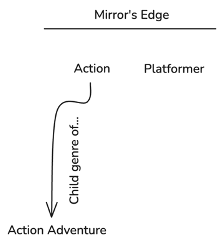
\includegraphics{mirrorsEdgeGenres}
		\centering
		\caption{A diagram showing the genres of Mirror's Edge}
	\end{figure}
	
	Mirror's Edge has numerous mechanics that it is famous for, such as wall jumping and wall sliding. These mechanics allow for adding complexity to the level design and make the game more interesting as the player can do more actions to complete a level.
	
	For my game I would model my game towards the platformer genre and the action genre.
	
	\subsection{Platforms}
	I am planning to build my video game for the x64 CPU architecture for Windows and the x64 CPU architecture for Linux. Though Linux can run Windows executables through the \href{https://www.winehq.org}{Wine} and forks of that such as \href{https://github.com/ValveSoftware/Proton}{Valve's Proton} translation layer, I'd like to also experiment with making builds for Linux as well.
	
	I am not planning on releasing my game with VR support or mobile support as it would be too time consuming to add support for these, as both of these input devices are very different from the one I'm targeting (Keyboard and Mouse).
	
	\newpage
	\subsection{Target Audience}
	My target audience is someone who is interested in parkour and action games. From my research, they are 13.6\% more likely to be male, \cite{gameTreeIndustryReports} from the US, \cite{gameDiscoverCoCountryBreakdown} and owns a computer with the specifications of:
	\begin{itemize}
		\item Windows 11.
		\item 16GBs of RAM.
		\item A 6-Core CPU with a clock speed of 2.495GHz.
		\item An NVIDIA GeForce RTX 3060 GPU with 8GBs of VRAM.
	\end{itemize} \cite{steamHardwareSurvey}
	
	\section{Game play and Mechanics}
	\begin{note}
		\textbf{Note:} Due to an unexpected cyber attack against the school network, essential services were down. These services being down caused students to lose the ability to do their school work. To make up for this, the games department reduced the scope of the brief to one where you only have to make the level. So, many of the mechanics are missing from the build of the game. The mechanics listed here were the \textbf{proposed} mechanics before anyone had any idea of a cyber attack.
	\end{note}
	\subsection{Gameplay Loop}
	The gameplay loop consists of doing a parkour level and being brought back to the start if the player has hit a fail condition (E.g. the player jumped of a surface) or if the player has decided to reset the level through a menu. This repetition of playing the same course over and over again until their successful final run gives the player fulfilment once they have finished their final run.
	\newpage
	\subsection{Controls}
	The controls are pretty simple and most mechanics are done automatically as the user plays the game.
	
	\begin{figure}[h]
		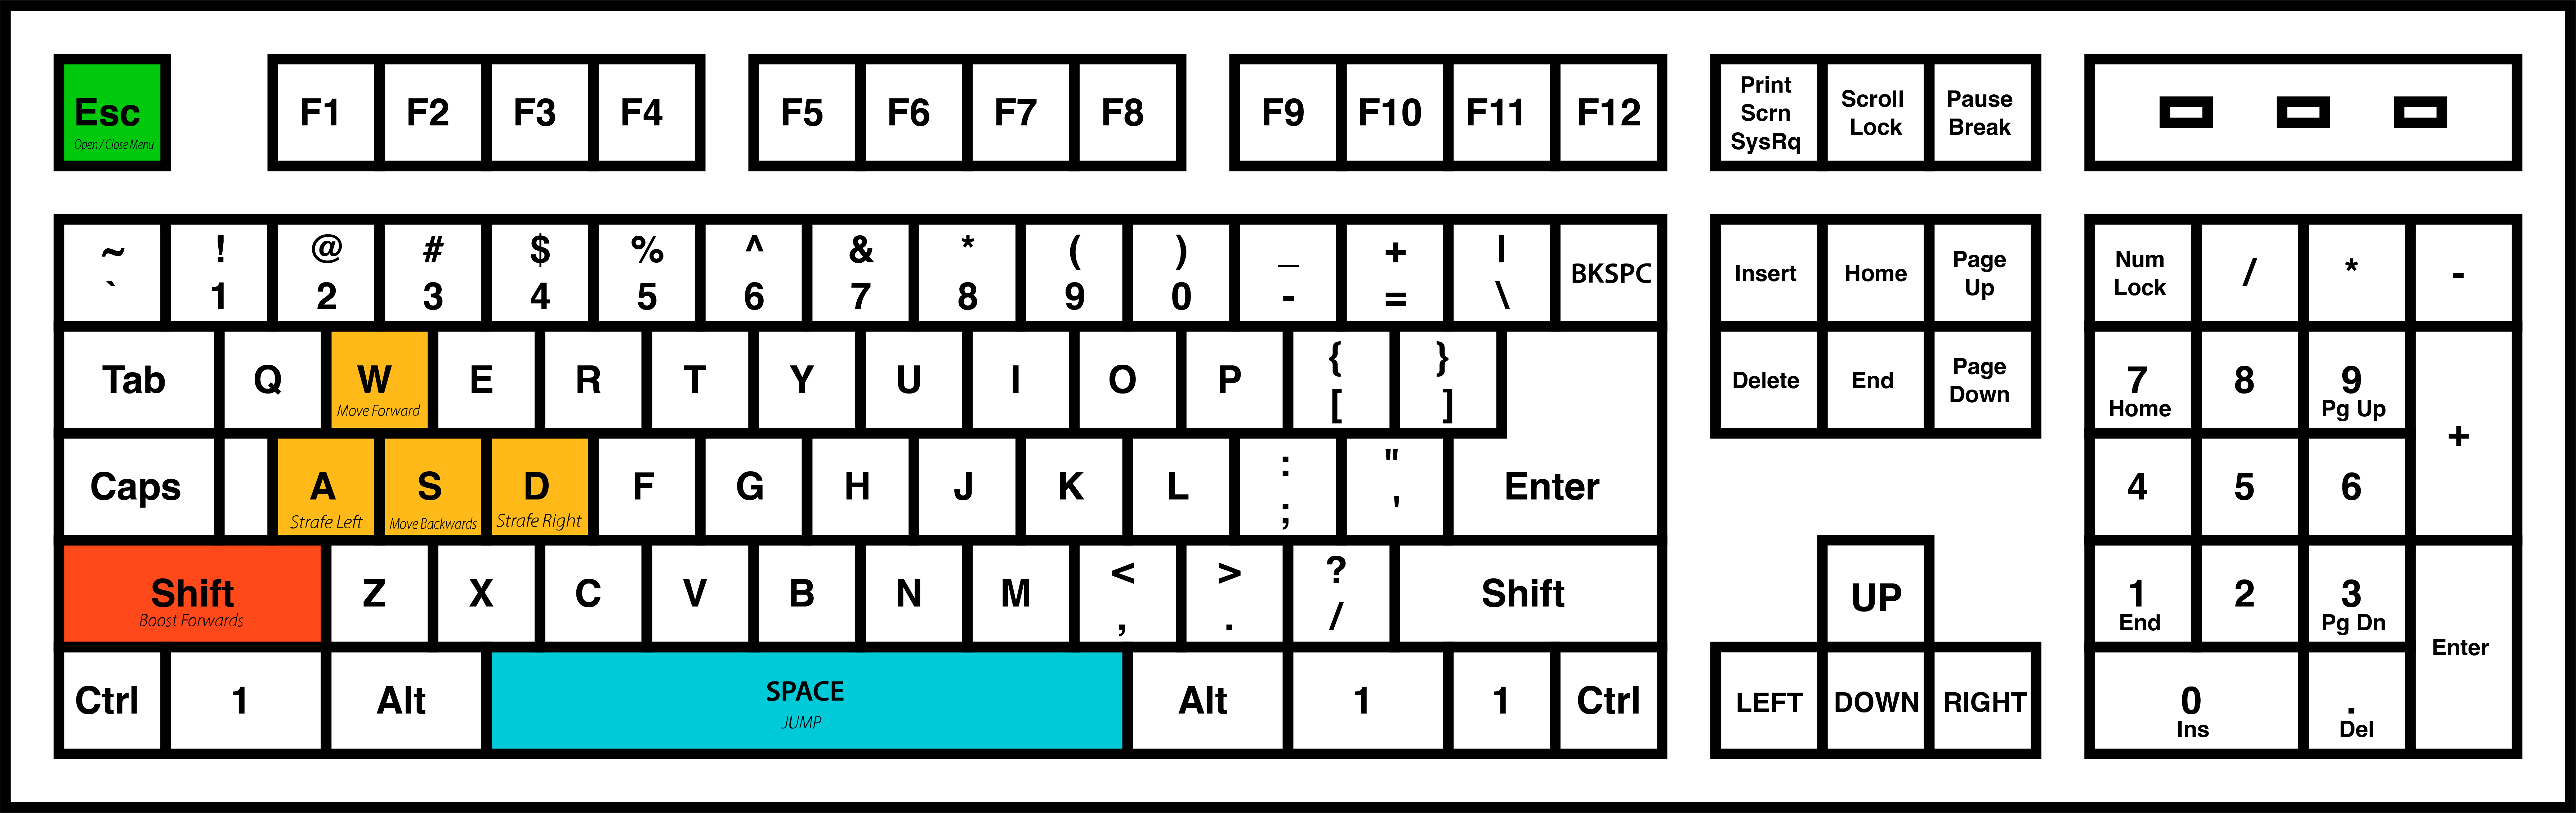
\includegraphics[scale=0.2]{keyboardLayout}
		\centering
		\caption{An annotated keyboard with the specific actions shown on each key}
	\end{figure}
	
	I am not planning to add controller support into the game.
	
	\subsection{Player Abilities}
	The player has multiple abilities (bar the regular movement):
	\begin{itemize}[]
		\item Boost \keystroke{SHIFT} - The player can add some momentum in the air by hitting the \keystroke{SHIFT} key. This, along with a jump, via the \keystroke{SPACEBAR} key, propels the player further.
		\begin{figure}[h]
			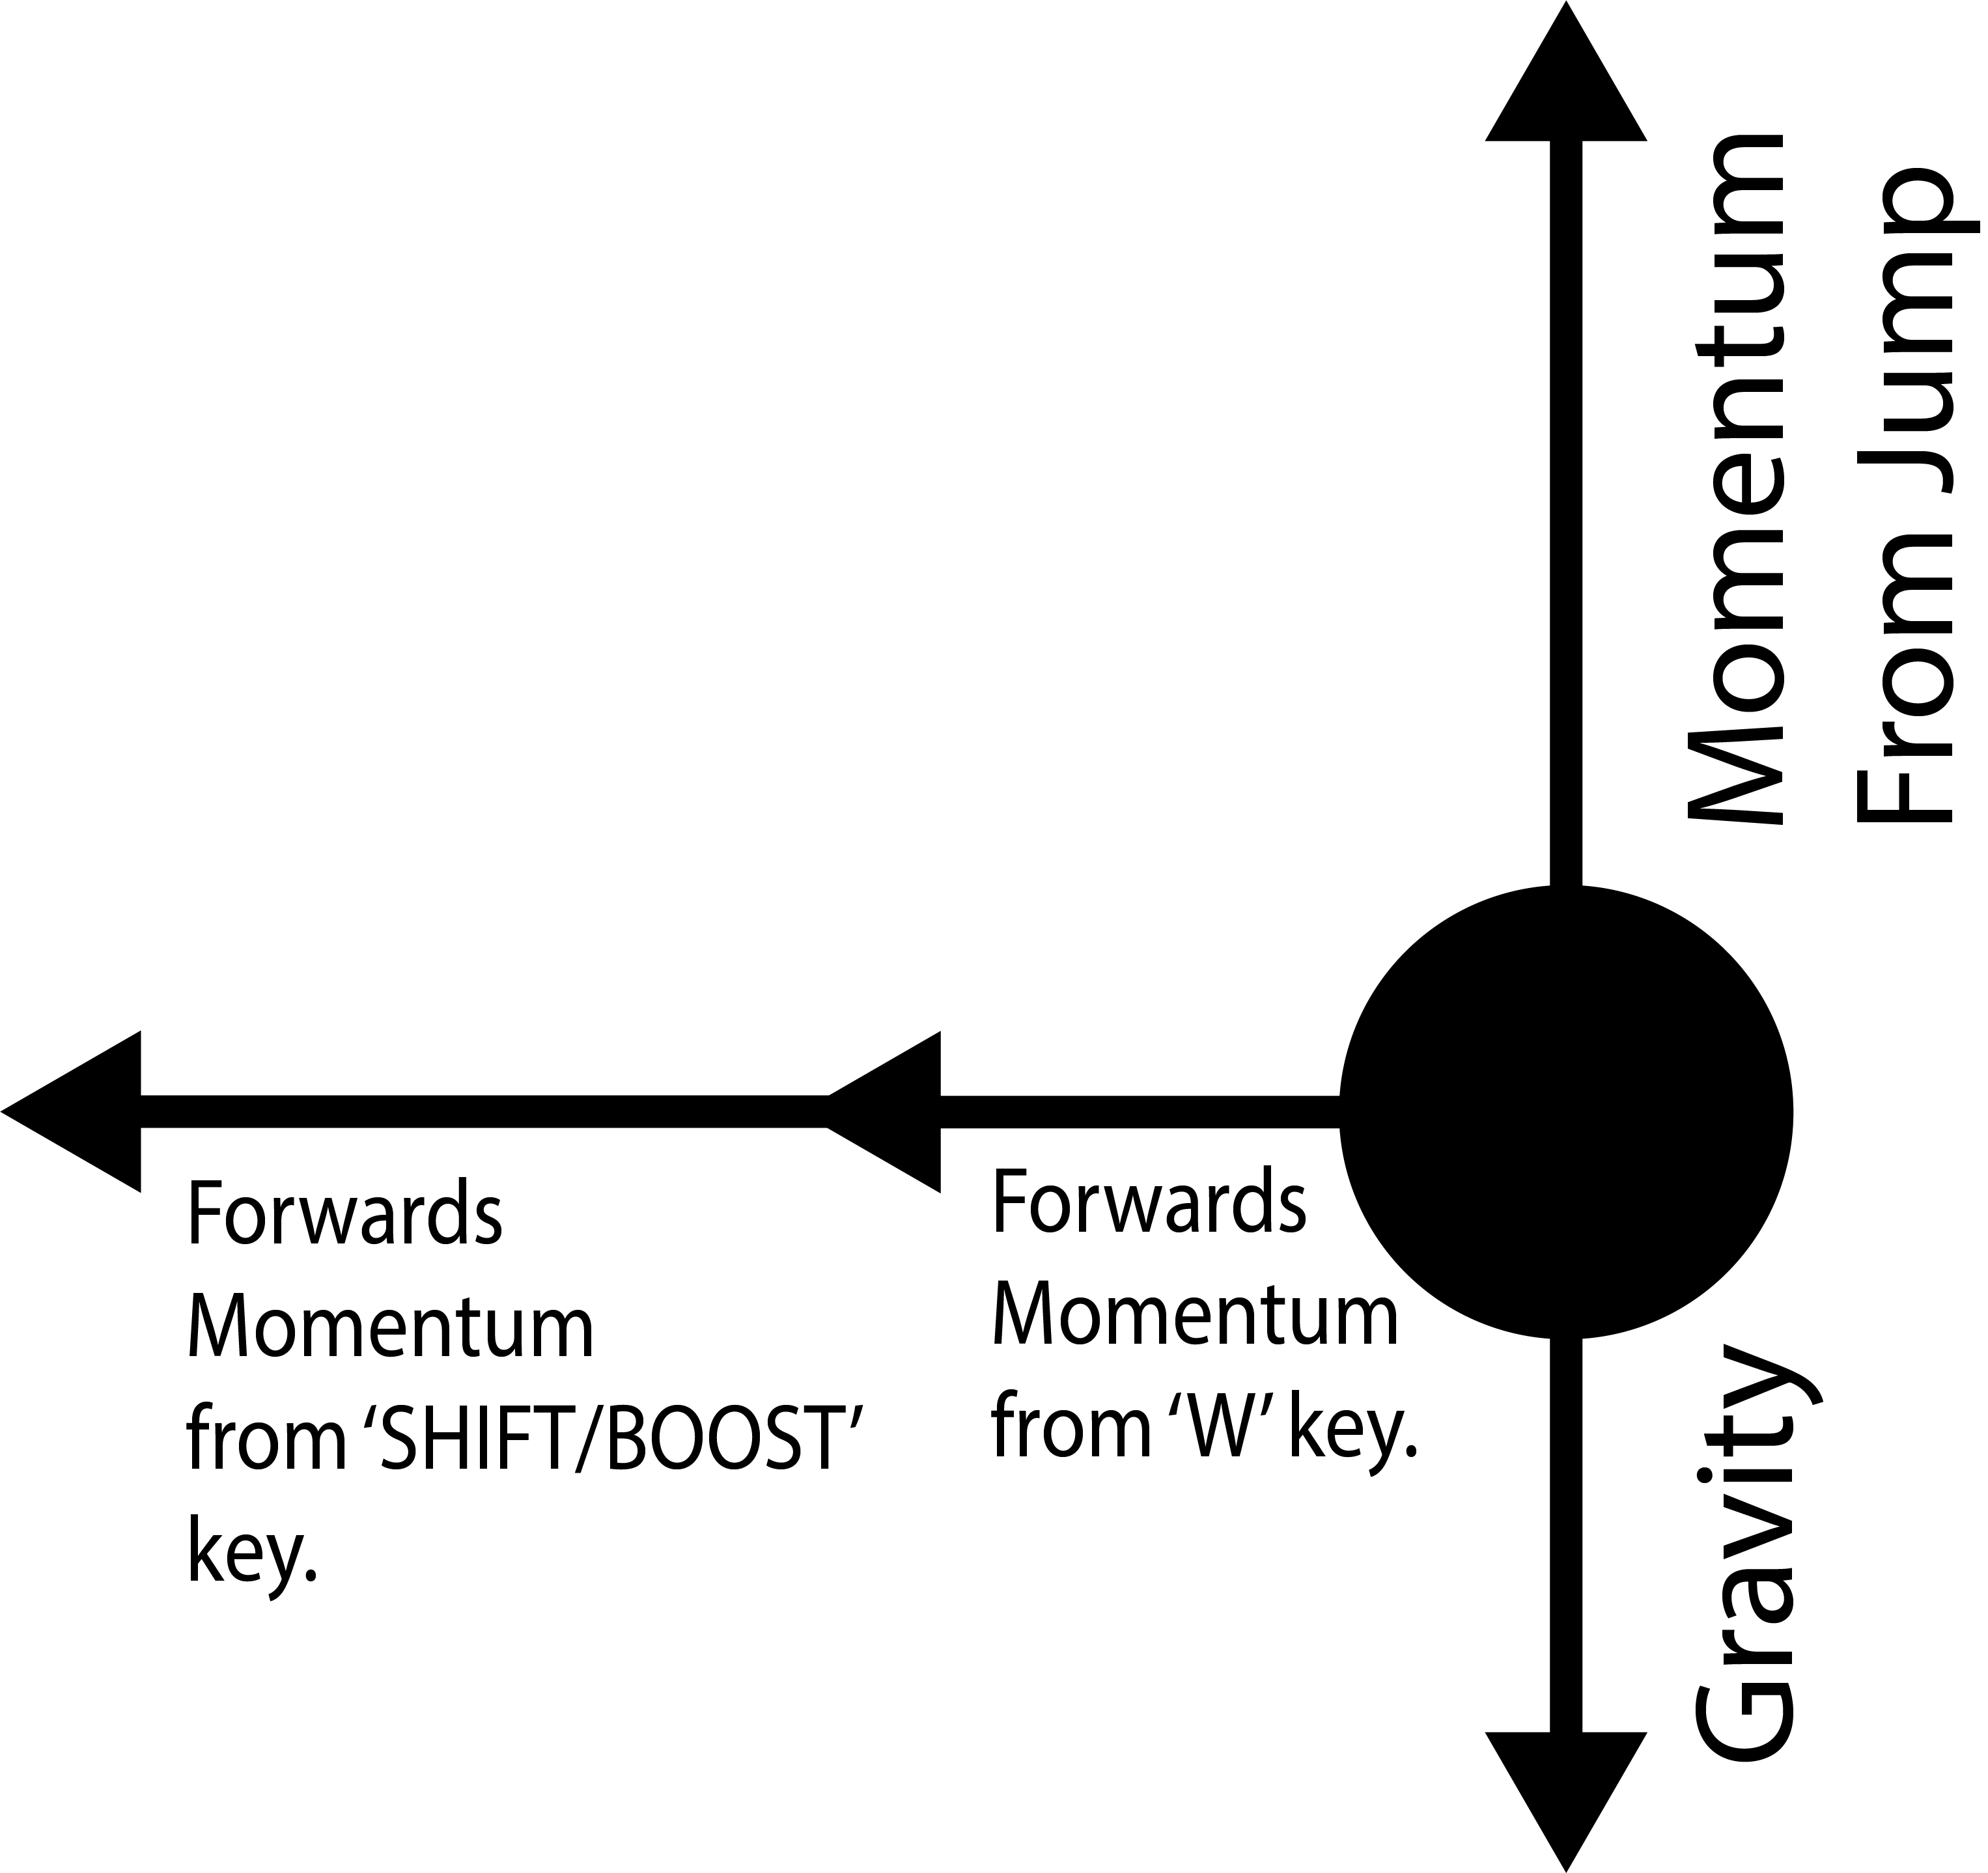
\includegraphics[scale=0.2]{jumpAndBoostForces}
			\centering
			\caption{The forces that are applied on the player when they jump and use the boost mechanic at the same time}
		\end{figure}
		\newpage
		\item Sliding \keystroke{N/A} - The slide mechanic allows for players to pick up speed along downward slopes. The player can use their mouse to control the direction of the slide. Sliding only works if the angle is in a goldilocks zone of angles.
		\begin{figure}[h]
			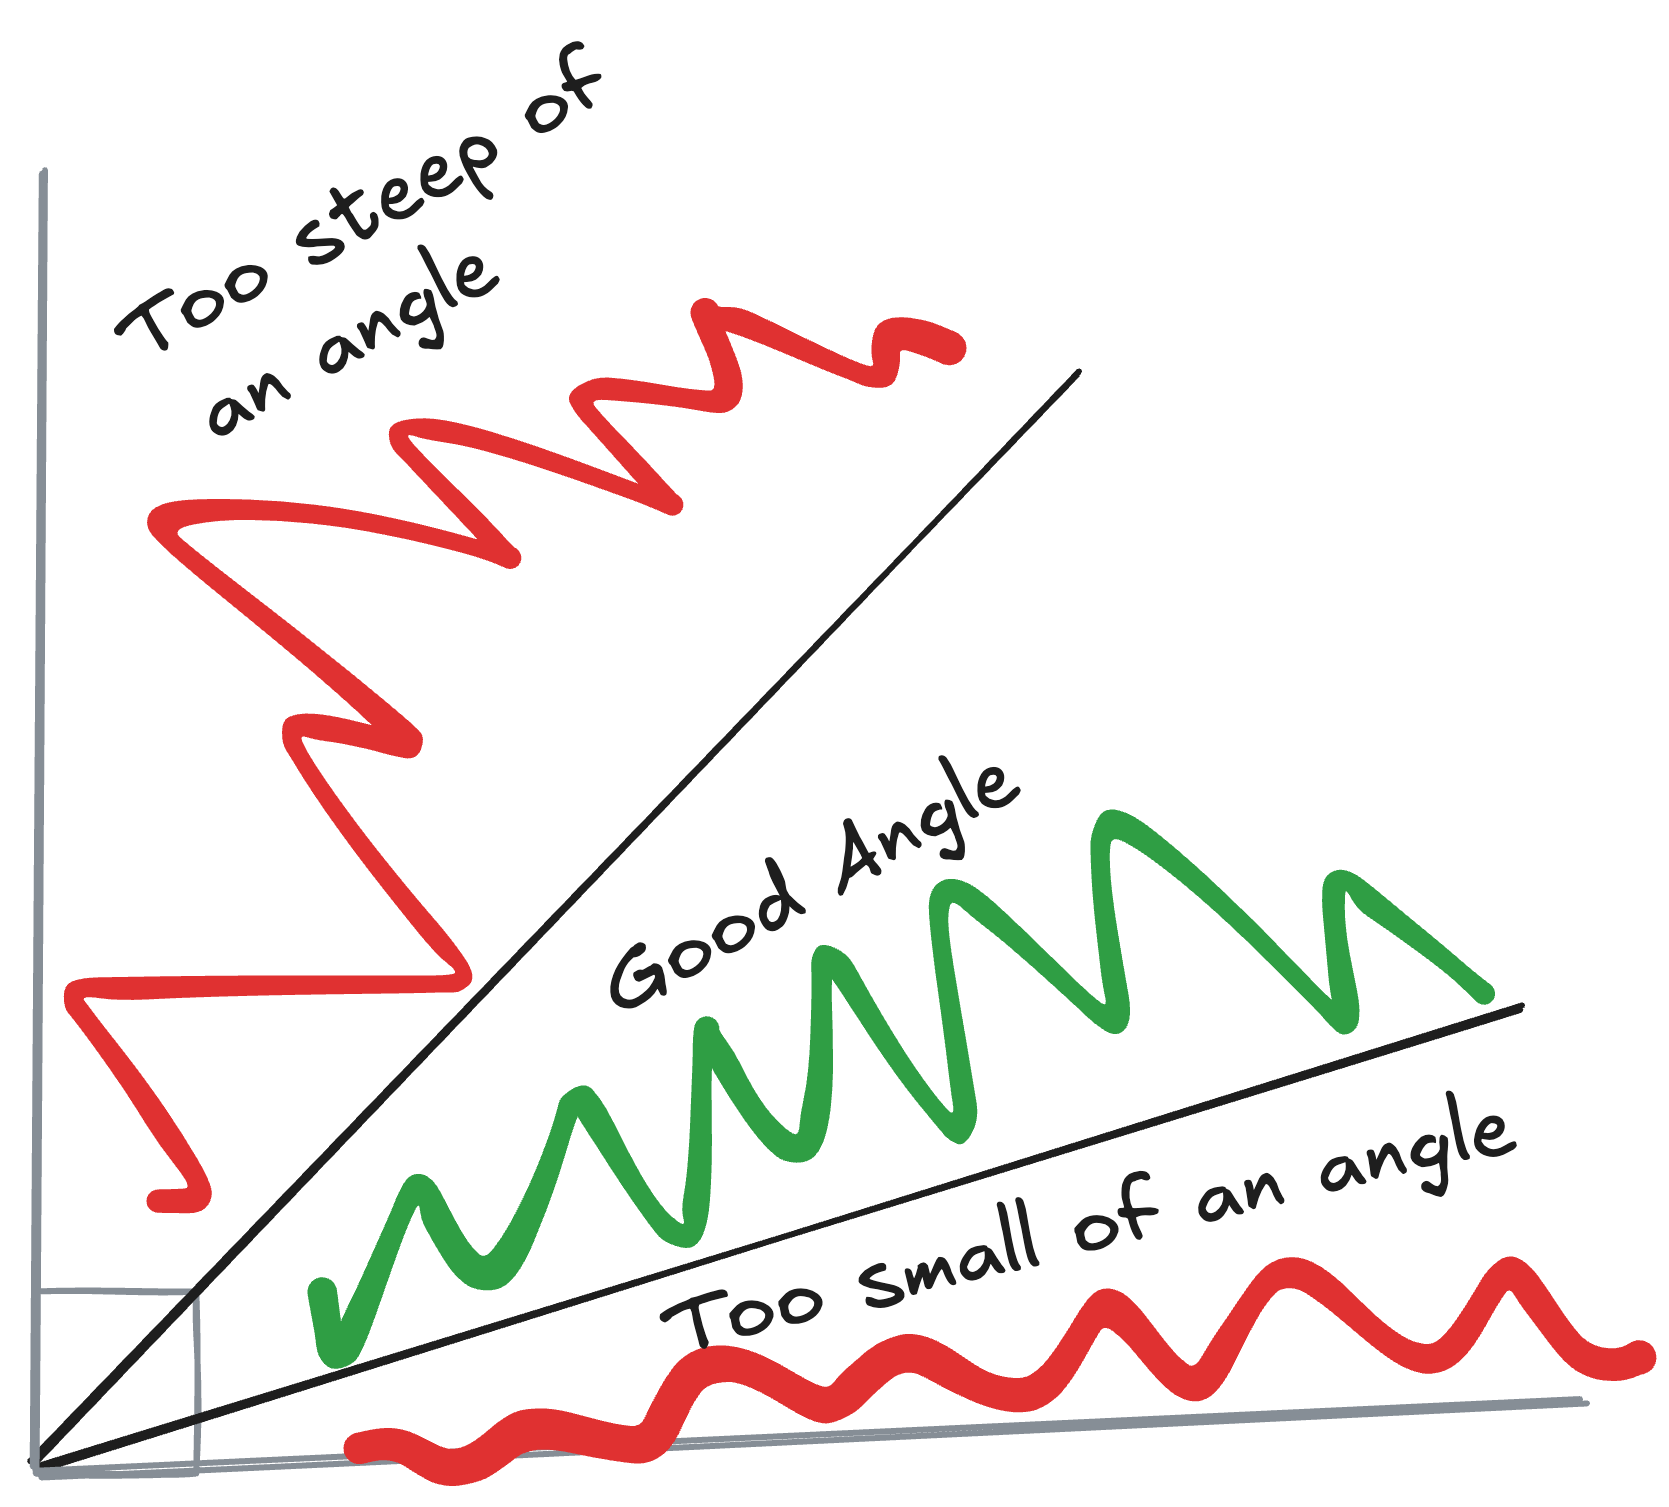
\includegraphics[scale=0.1]{angleSteepness}
			\centering
			\caption{A diagram showing "good angles" and "too steep / small of an angle".}
		\end{figure}
	\end{itemize}

	\subsection{Difficulty and Progression}
	The games difficulty is more or less constant, bar the tutorial, the game sits at a medium difficultly. If the game is too easy, it would not feel as good when the player completes a level and, if it is too hard, the player will feel frustrated.

	There are a number of variables that I could use to change difficulty:
	\begin{itemize}
	  \item The walk speed.
	  \item The amount of time that the Boost mechanic takes to regenerate.
	  \item The spacing between platforms.
	  \item The amount of speed that sliding down a surface generates.
	\end{itemize}

	\section{Level and World Design}

	\subsection{Level Structure}
	All levels have a starting point and an ending point. There will be multiple routes to get from the starting point to the ending point. The different routes could expose different parts of the map to the player which would increase player replay ability and would give the player more choice on where to go. There is a main menu which will act as a way to pick levels, and this level selector will only allow you to pick levels based on if the previous level has been completed or not.


	\subsection{Environments and Biomes}
	Before I learnt about the IT outage, I was planning on building multiple levels to make sure I got a good a good grade. I was planning on building two levels:
	\begin{description}
	  \item[A sandy, desert level.] This was the first level that I made, and the only level I made in the end due to the IT outage. The reason I picked this level out of the two to make is that it is easier to make then the other way especially if I made it in a smart way. The smart way I used to make the sand dunes is to use a depth map. Which allows you to have an greyscale image define the depth of an object. Where blacks are lower down in the mesh and lighter colours / whites are higher up in the mesh. For example here is the depth map I used:
			\begin{figure}[h]
			  \includegraphics[scale=0.09]{desertHeightMap}
			  \centering
			  \caption{A depth map}
			\end{figure}
	  \item[An abandoned factory level.] This was the second level I was planning to make, it was heavily inspired by the games Portal 1 and Portal 2. The level was going to have overgrown plant life and be a neglected building with cracks on the wall.
	\end{description}
	
	\section{Art and Aesthetics}
	\subsection{Art Style}
	I am trying to aim for a realistic art style as that is one of Unreal Engine's specialities. This means I will be using models with high polygon counts, however low-quality LODs could be used as for a lot of the time the player will be far away from the objects.
	\subsection{UI/UX Design}
	\begin{figure}[h]
			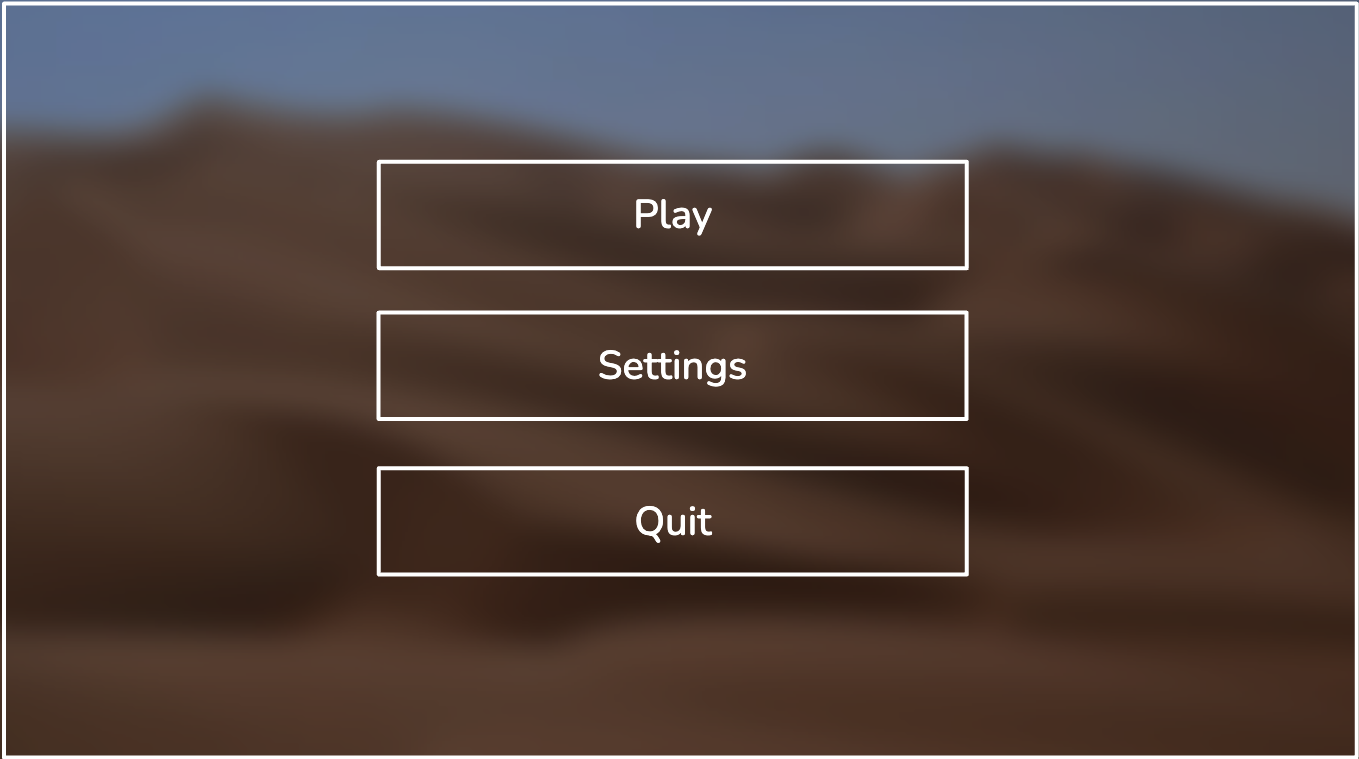
\includegraphics[scale=0.3]{mainMenu.png}
			\centering
			\caption{The main menu}
	\end{figure}
	This was my main idea for the user interface for the game, it would have buttons for starting the game, entering the settings and quitting the game. I was thinking about having the background being a video of the games levels; darkened and with a gaussian blur.
	
	Hitting the \keystroke{Escape} key will take you back to this screen whilst in a level.
	\newpage
	\begin{figure}[h]
			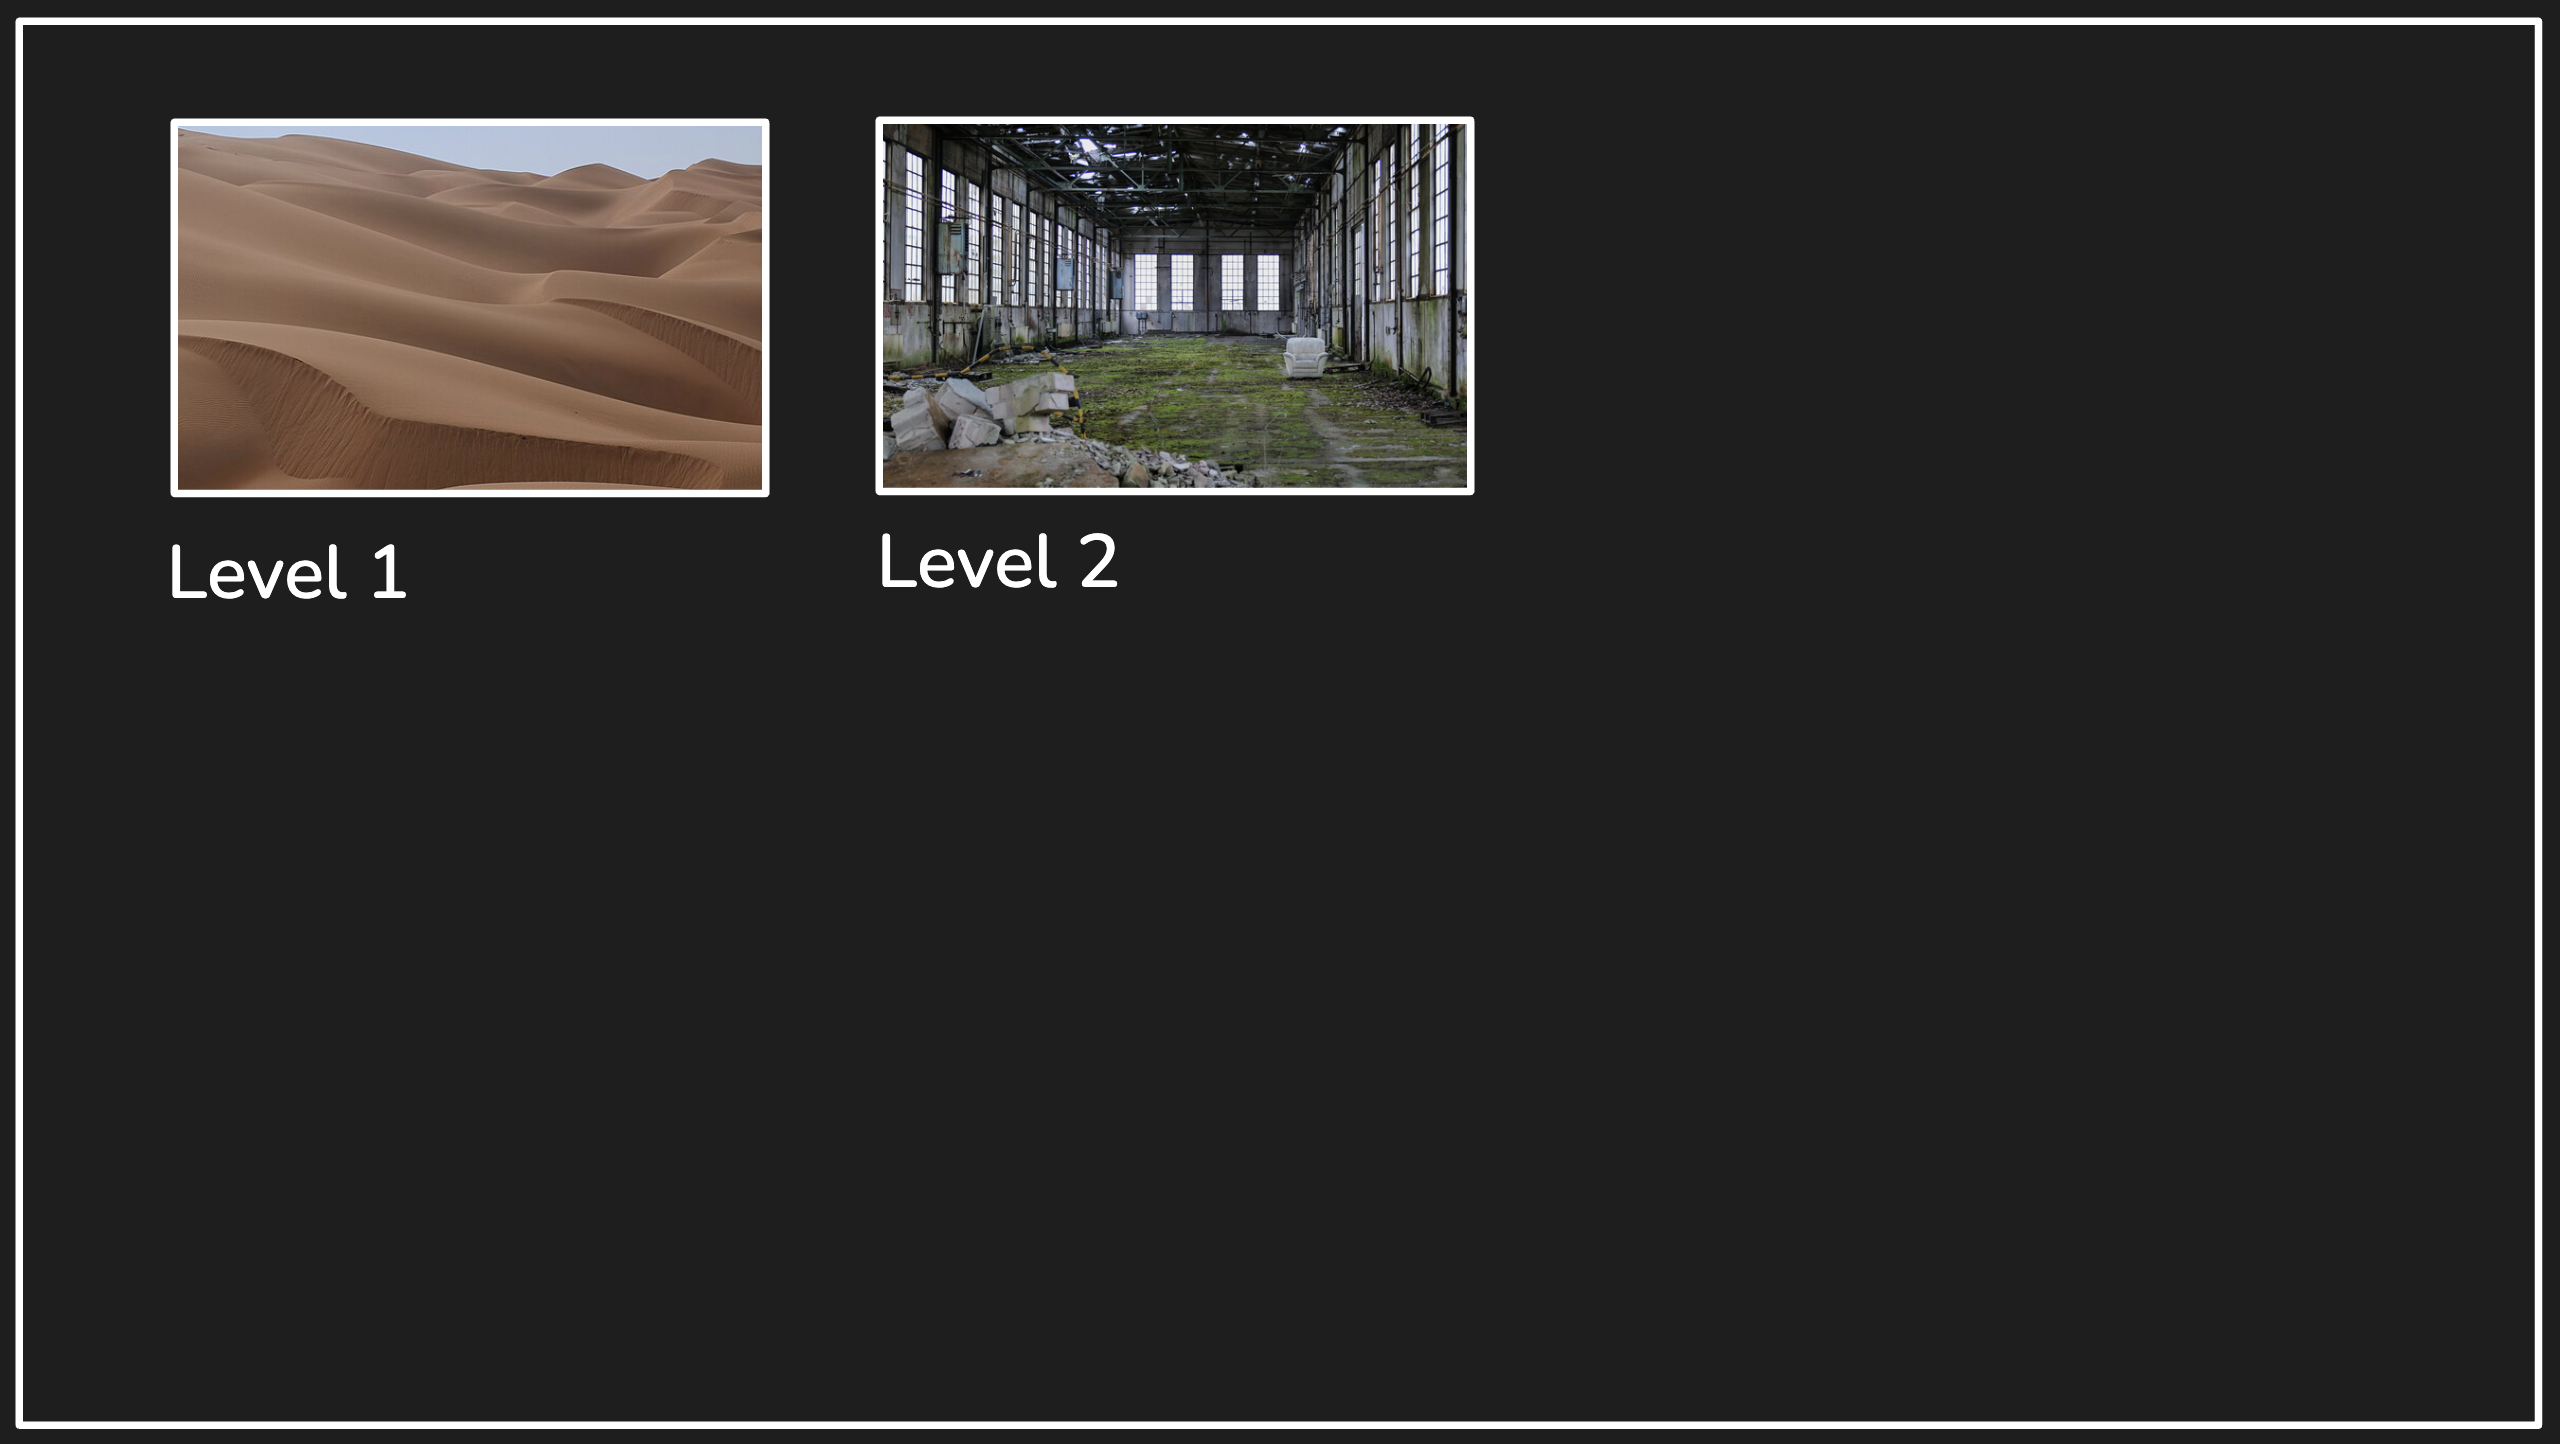
\includegraphics[scale=0.3]{levelSelect.png}
			\centering
			\caption{The level selector}
	\end{figure}
	Each of the levels are selectable within the UI and once they are clicked they are loaded. Currently, the images for the level selector are just placeholder images. They would be replaced by actual images of the level once the game is done.
	\begin{figure}[h]
			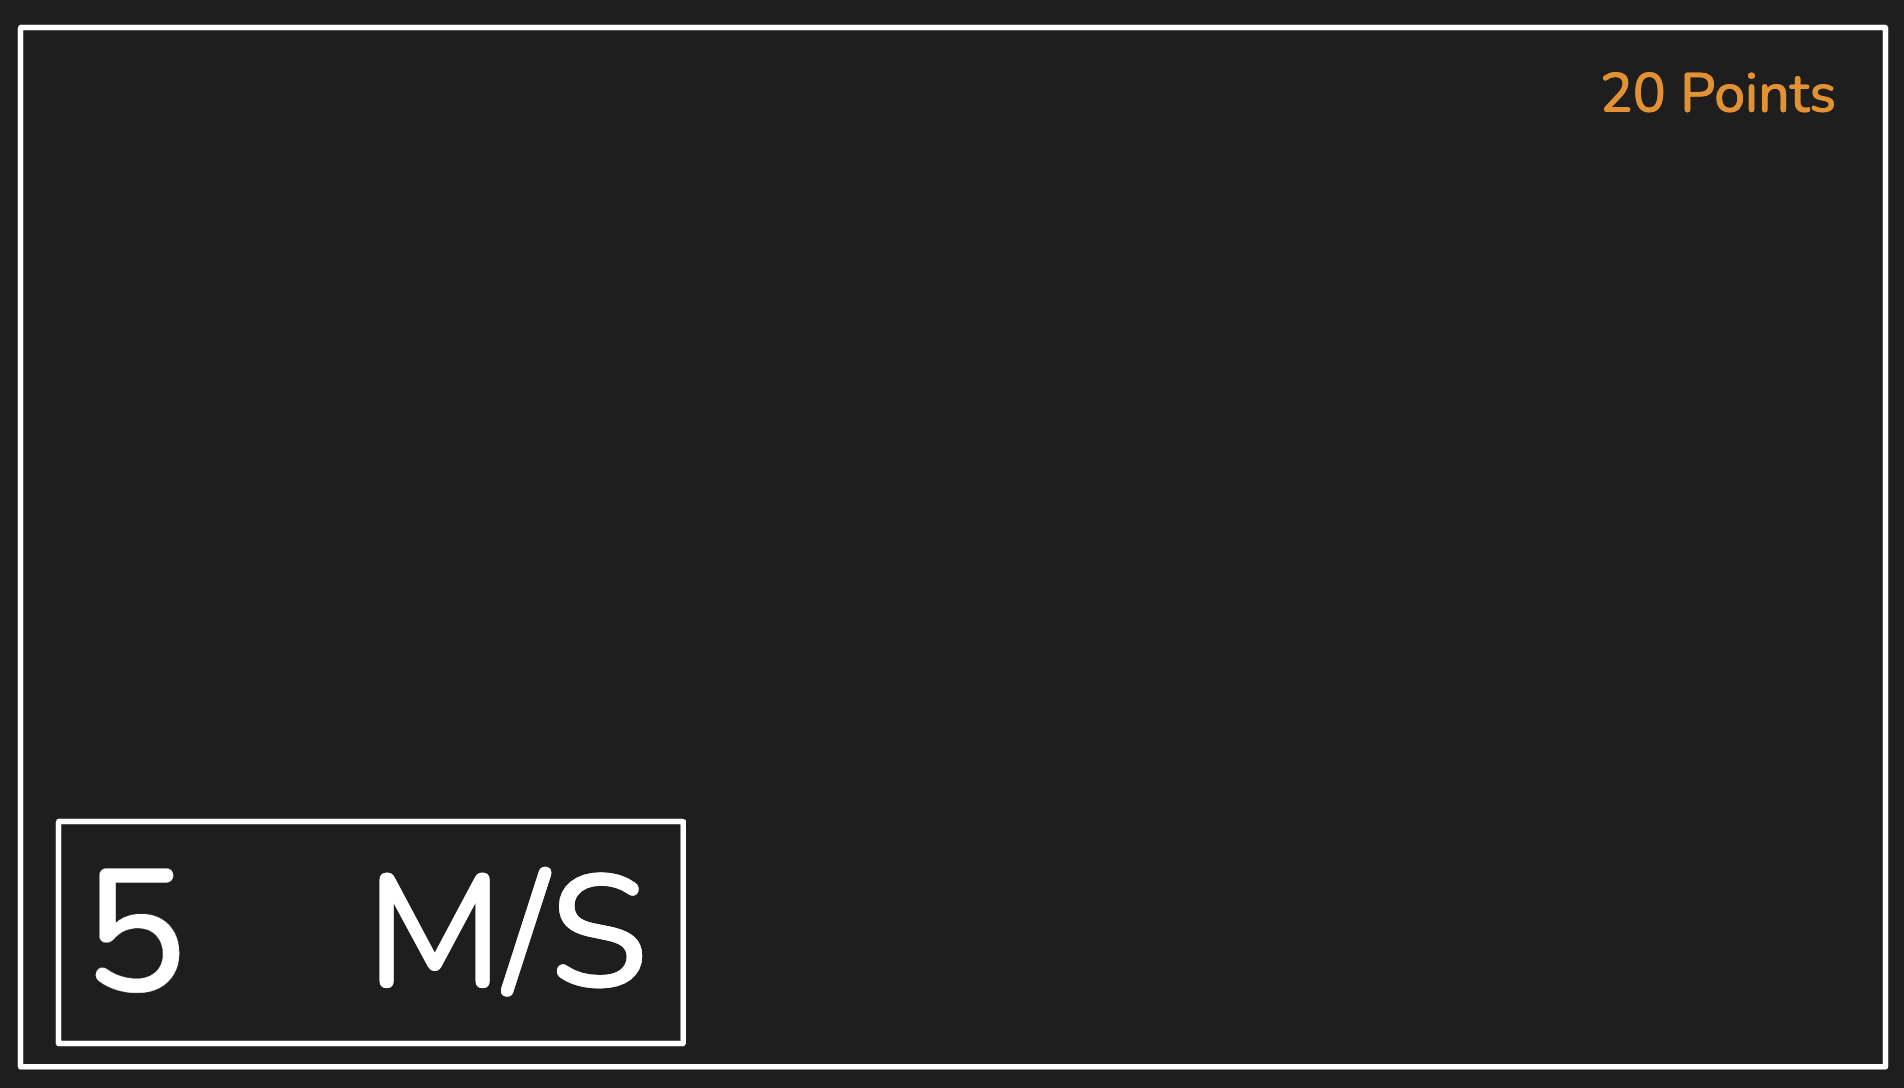
\includegraphics[scale=0.365]{inGameUI.png}
			\centering
			\caption{The in-game UI}
	\end{figure}
	
	The in-game UI has 2 major elements. The current speed of the character and the current amount of points. This part of the UI is redrawn and re-calculated on every new frame.

	\subsection{Mood Boards}
	Here are some photos I was inspired by:
	\subsubsection{Level 1: Sandy Desert Level}
	\begin{adjustbox}{%
    	max totalsize={\linewidth}{\textheight},
    	frame
	}
		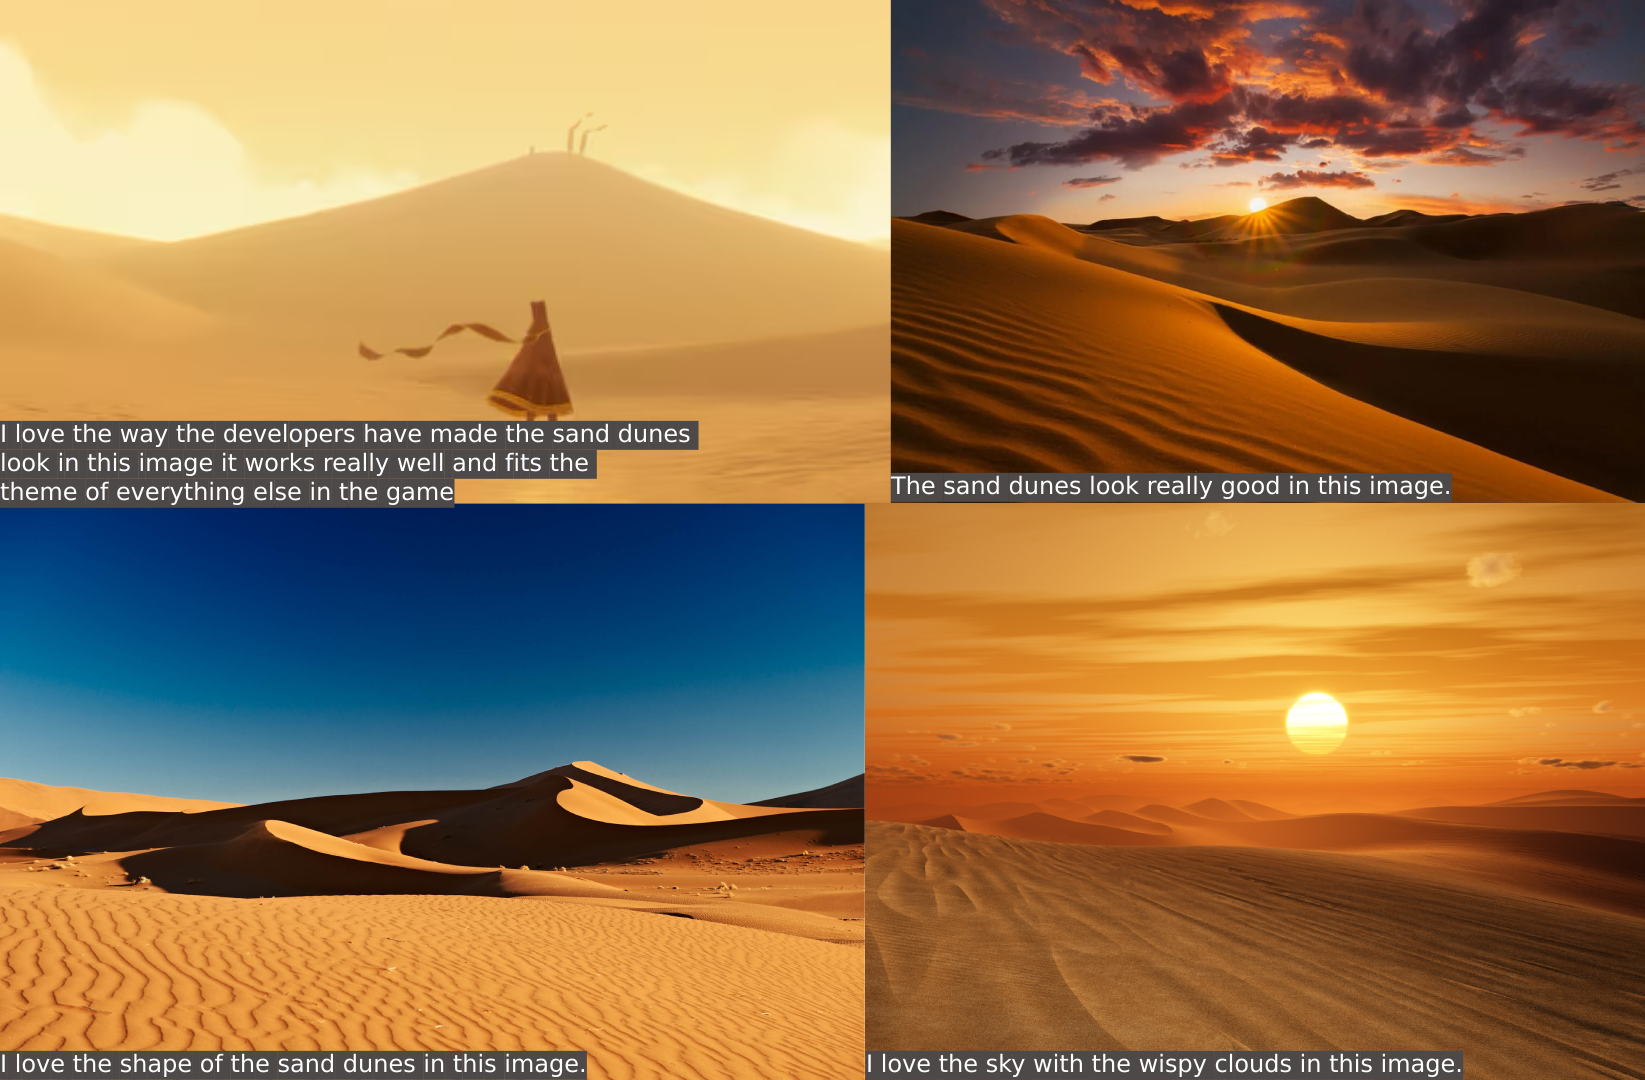
\includegraphics{desertMoodboard.png} 
	\end{adjustbox}
	
	\subsubsection{Level 2: Abandoned Factory Level}
	\begin{adjustbox}{%
    	max totalsize={\linewidth}{\textheight},
    	frame
	}
		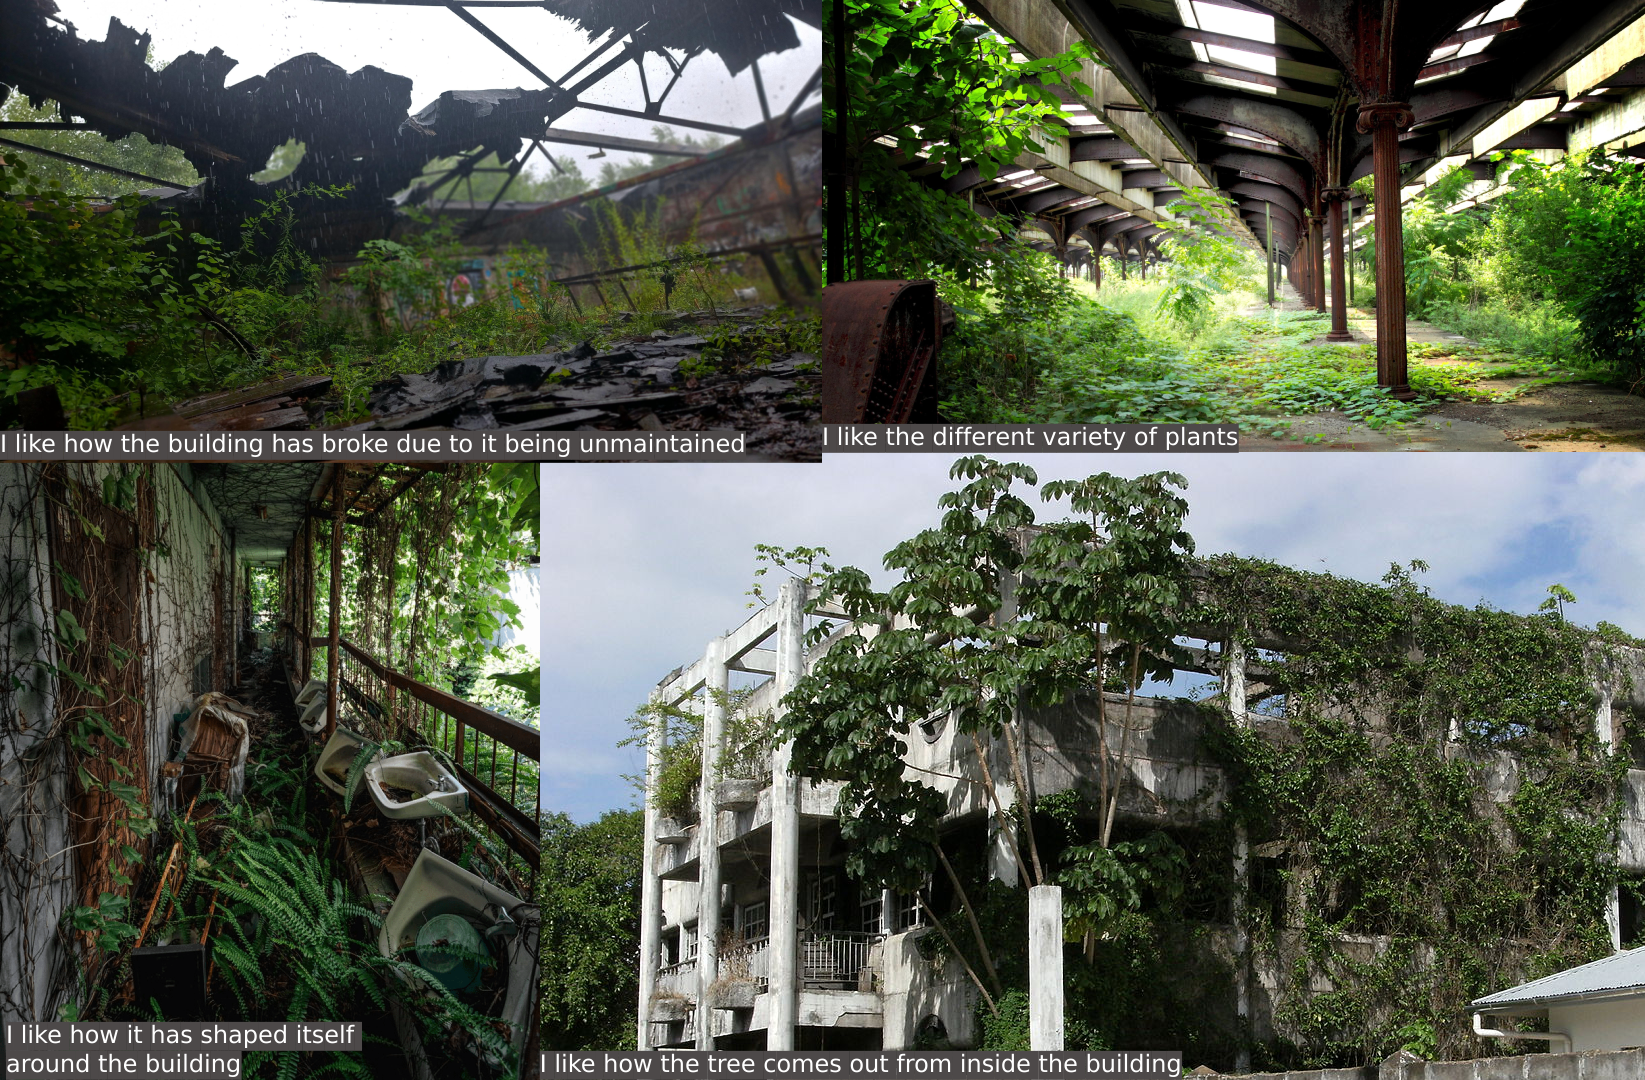
\includegraphics{factoryMoodBoard.png} 
	\end{adjustbox}
	
	\subsection{Initial Sketches}
	Here are some sketches of my work:
	
	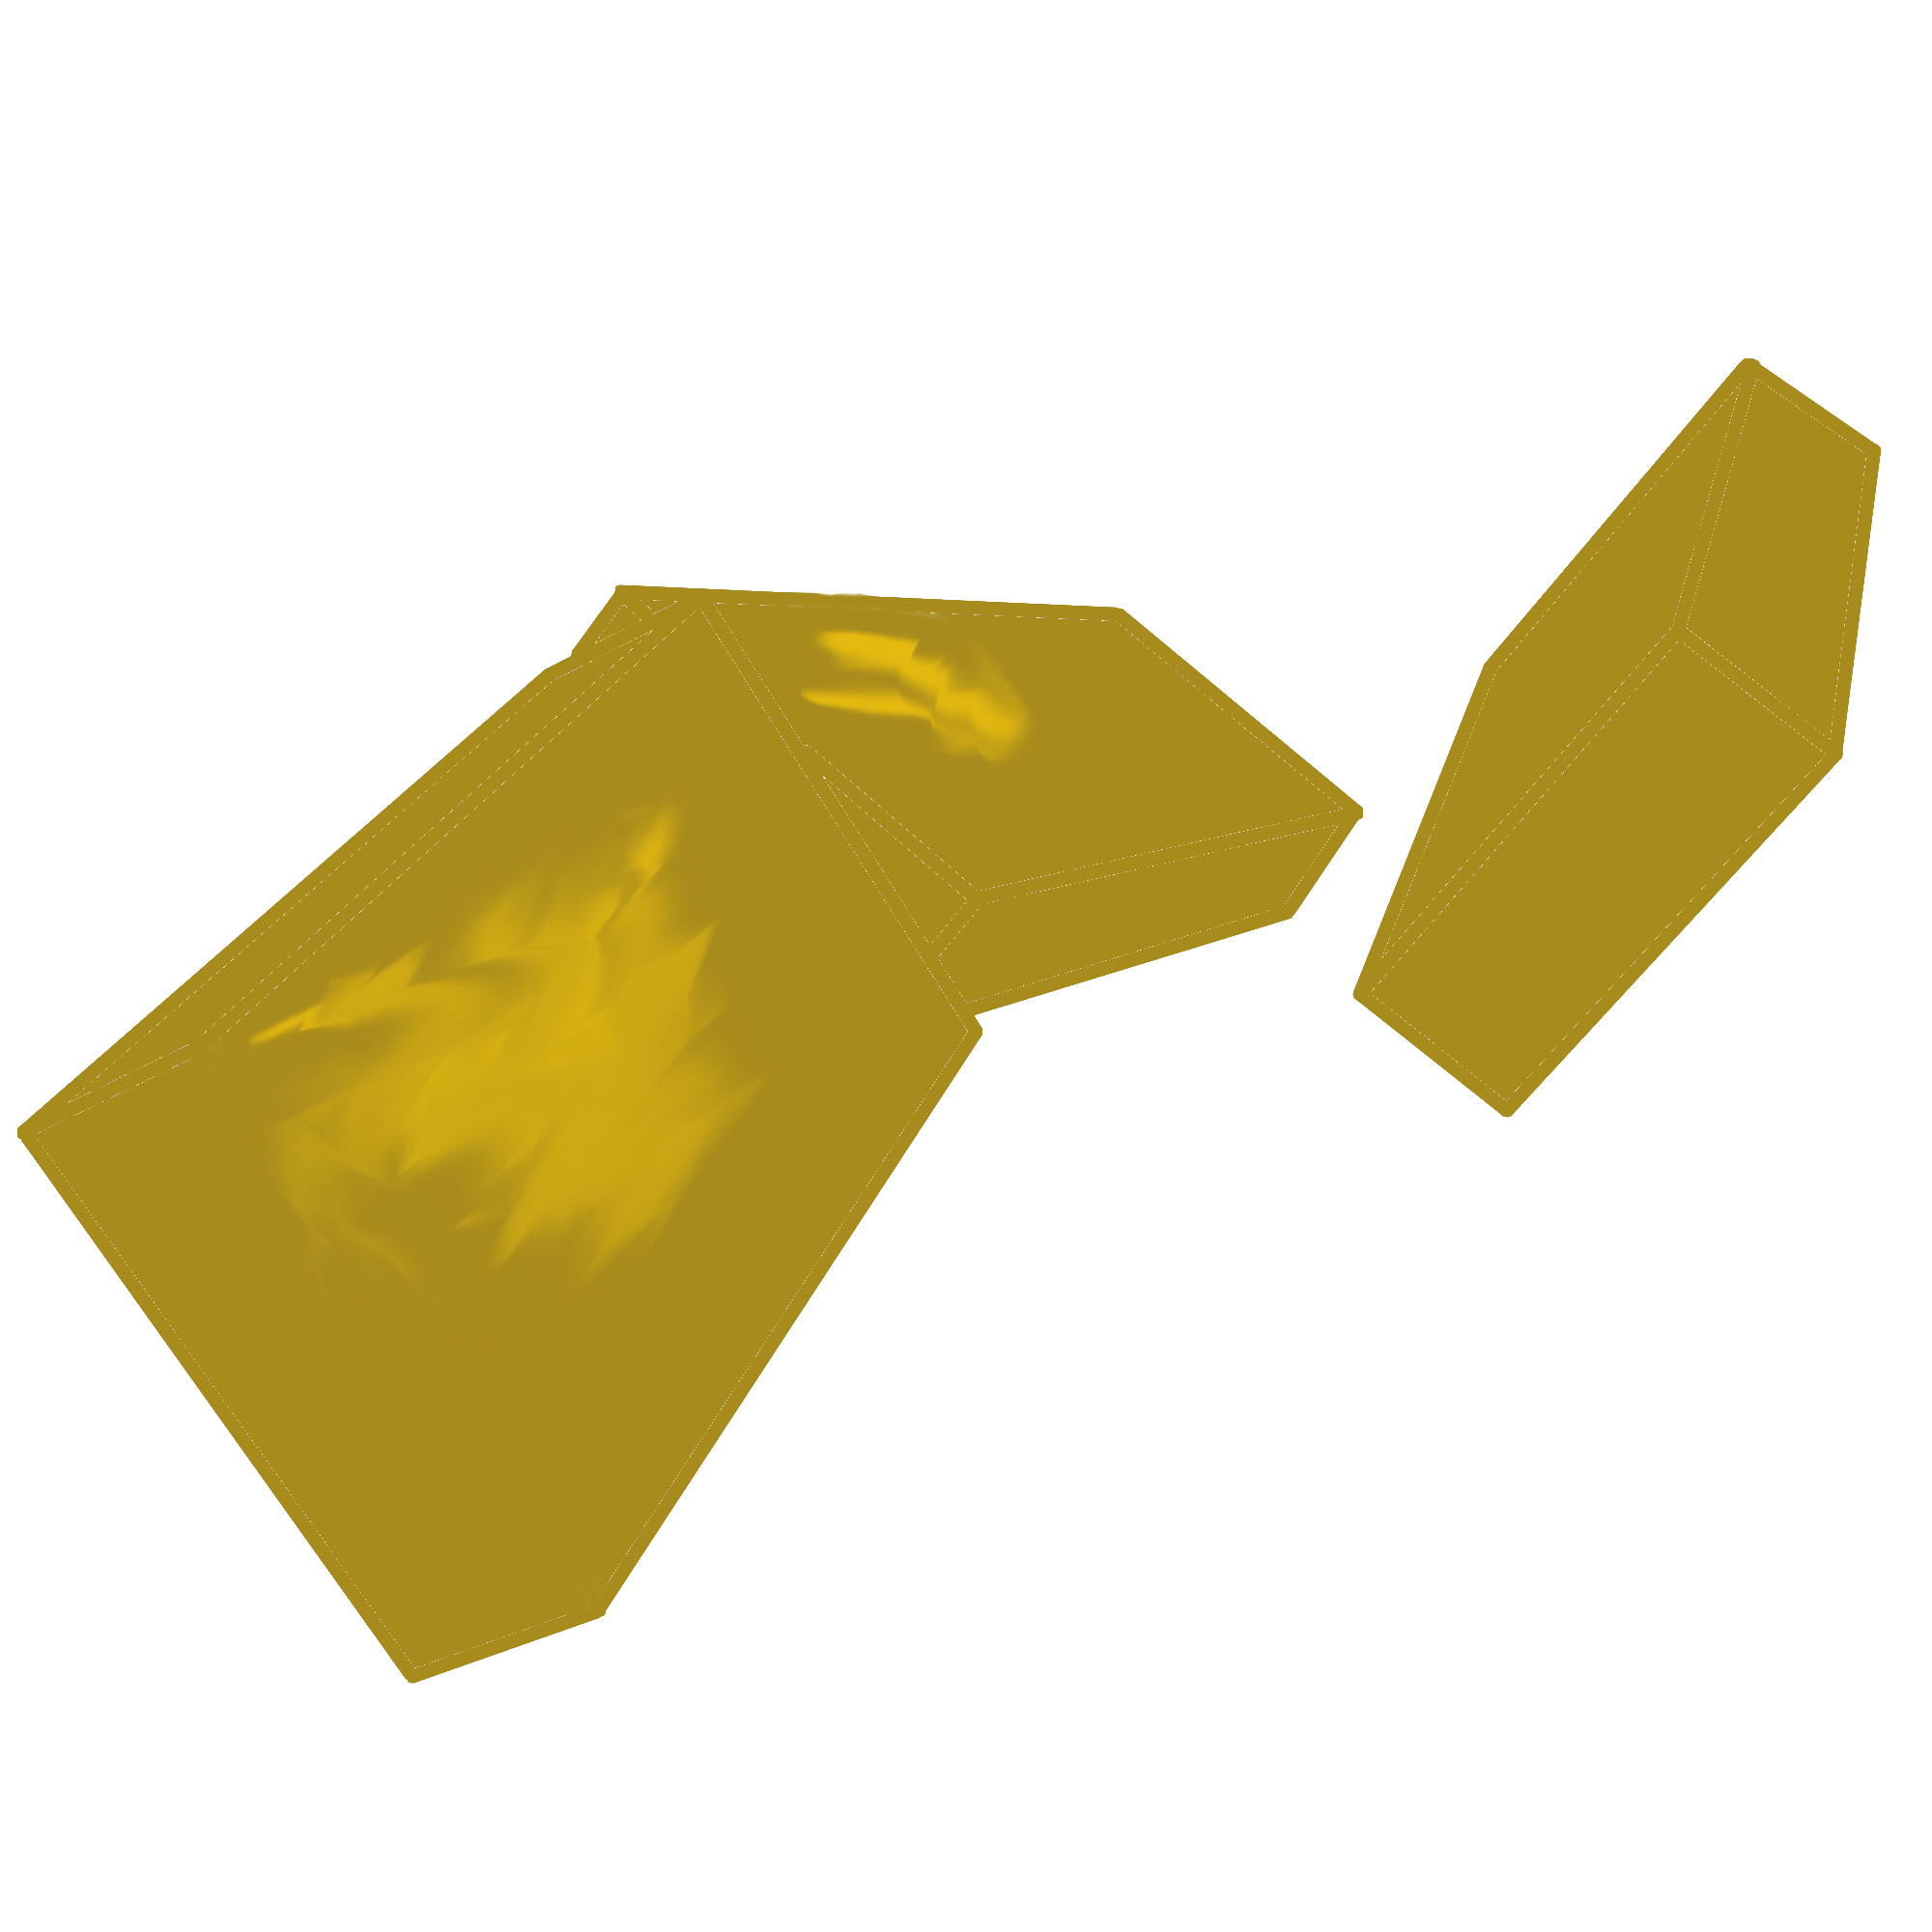
\includegraphics[scale=0.1]{platforms.png}
	
	
\includegraphics[scale=0.1]{platformsTwo.png}
	
	\section{Audio}
	To make the gameplay a little more interesting I wanted to implement some music and sound effects. If I had some extra time to work on the project I would have implemented these.
	\subsection{Music Style and Technical Aspects}
 	One thing I am really inspired by and one thing I would love to make in this game is adaptive music. Adaptive music is a kind of music where the music changes based on what is happening in the game. For example, you could add or remove instruments or change tracks seamlessly. I would say the music genre for this game would be an electronic one with my major inspirations being from artists such as Daft Punk.
	\subsection{Audio Cues and Sound Effects}
	There will be a few click sounds effects for clicking on UI elements and a couple smashing sound effects when the player breaks parts of the level. These would be sourced from internet foley sources that have a open license. 
	\subsection{Technical Aspects}
	These would be played using UE5's \href{https://dev.epicgames.com/documentation/en-us/unreal-engine/metasounds-the-next-generation-sound-sources-in-unreal-engine}{Metasounds}. This way I can load in tracks and control audio using code. This also allows me to control the cardinal direction and, due to that, what speakers / pair of speakers play the actual audio.
	
	\section{Project Management}
	\subsection{Monday.com}
	I am using monday.com to act as a to-do list. Monday.com is good as it allows for you to visualise your tasks as a gantt chart.
	\subsection{Github and Git}
	I am using Github to store my written work. After I make a change I can use git to create a commit (a store of my files in a point in time with a message to say what I have changed) and then push it of to Github (a place to store files tracked with Git). I can then get Github to turn my work into a PDF document using a YAML file and Github Actions. \href{https://github.com/dylanru-sm-college/A2-GDD}{Here} is a link to this text on Github.
	\begin{figure}[h]
			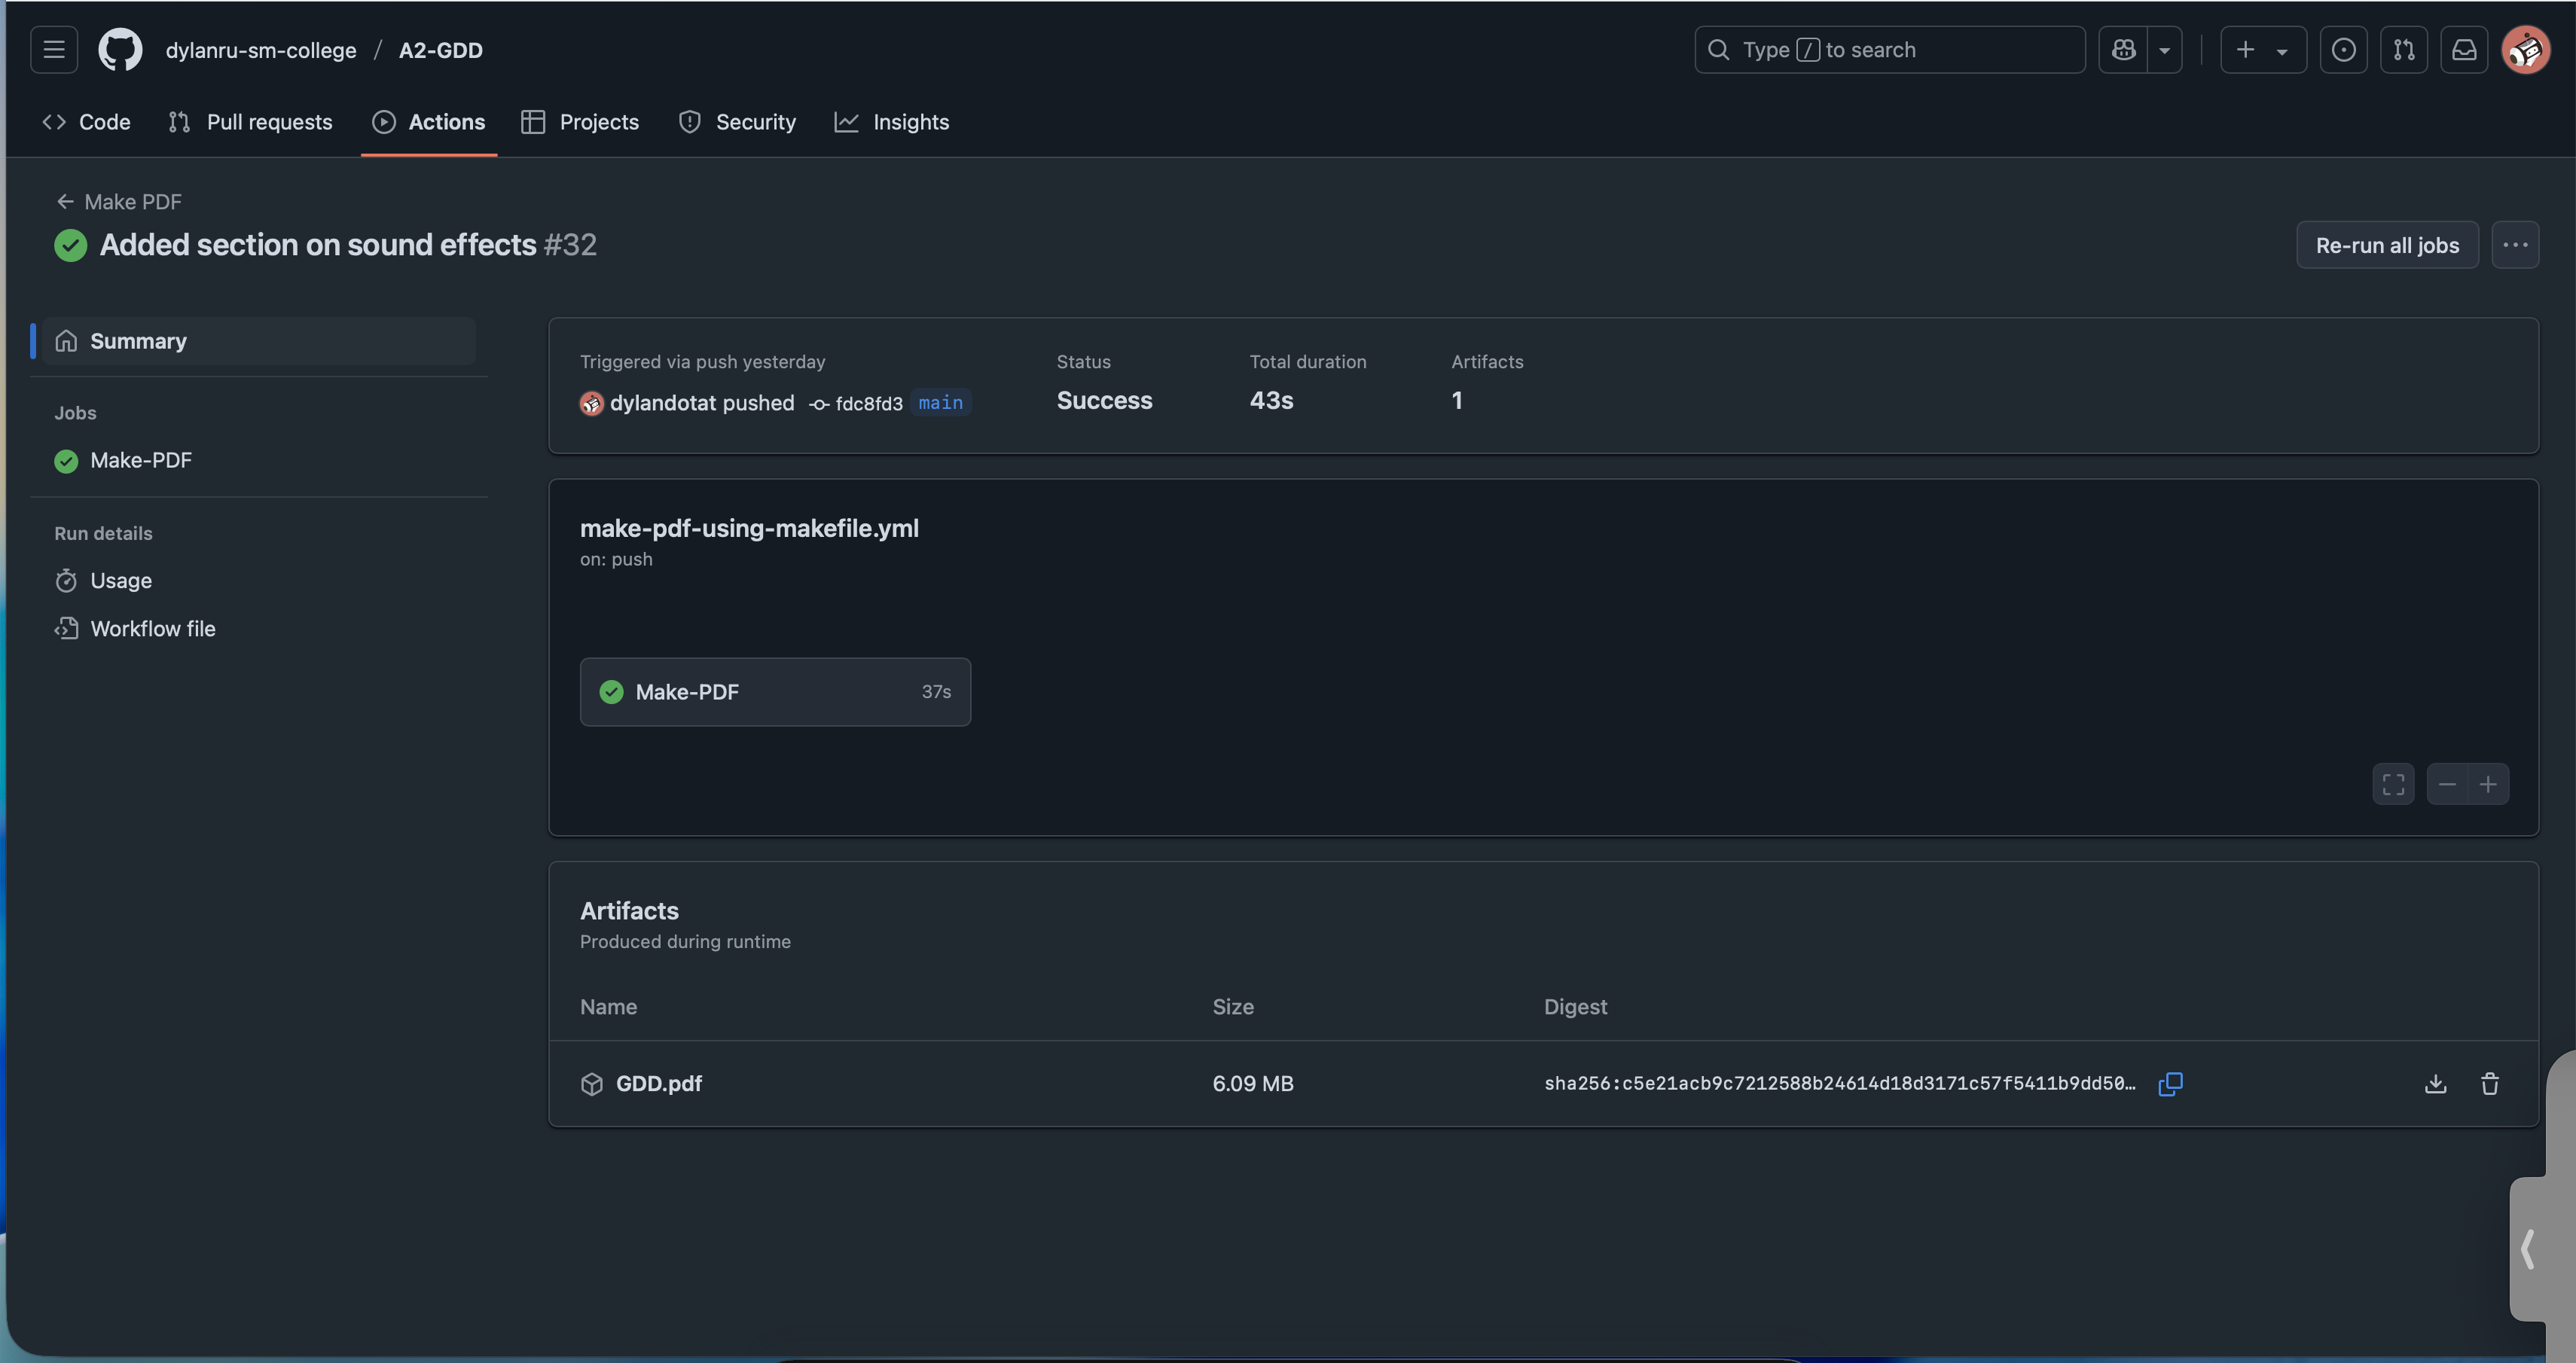
\includegraphics[scale=0.29]{githubActionsUI.png}
			\centering
			\caption{Github Actions compiling my work.} 
	\end{figure}

	\newpage
	{\setlength{\parskip}{0pt}%
	\bibliography{references}
	}
	
\end{document}
